\documentclass{../indiv}
\graphicspath{{../../images/part1/ch2/}}
\setcounter{chapter}{1}

\begin{document}
	\chapter{初始環境設定}
	\section{\LaTeX 的運作模式與編譯流程}
	先前提到\LaTeX 是一套功能強大且複雜的排版「系統」,顧名思義可知它並非一個獨立運行的程式,而是將每個獨立的小程式串成一組「編譯鍊」(Compile Chain),才得以支援這麼多自動化的功能。
	\begin{figure}[H]
		\centering
		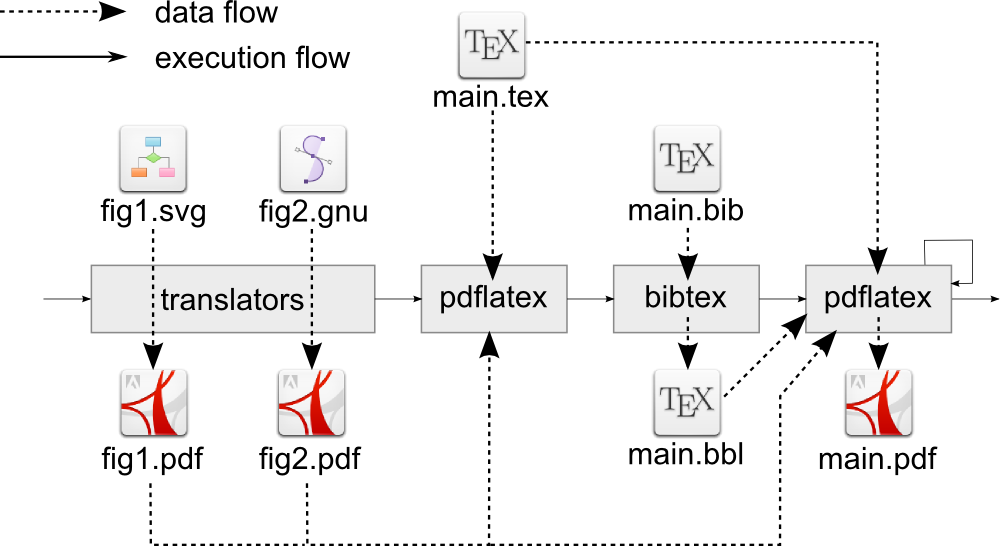
\includegraphics[width=0.6\linewidth]{process.png}
		\caption{一種典型的\LaTeX 文件編譯流程}
		\label{fig:Compile Process}
	\end{figure}
	一份文件的產出還必須仰賴許多字形檔、格式檔與額外的套件包,而套件包之間的相依性也往往非常複雜,不同的文件還可能會用到不同的編譯流程。因此,這些工具不可能讓我們一個一個安裝,因為保證還沒裝完你就會先累死。
	
	幸運的是,科技就是為了便利而存在。網路上早已有很多大佬設計的\TeX /\LaTeX 發行版(Disturbution),裡面就包含了那些最常用的工具,免去手動安裝的煩惱。而且它還有另一個最重要的功能,也就是會自動管理需要用到的套件,缺了什麼就幫你下載什麼,根本就是最偉大的發明之一了XD。(真不愧是號稱系統管理者的救世主)
	\begin{extra}
		\item 其實許多大型程式的開發也同樣必須透過一連串的工具達成,例如一套典型的開發環境可能會包含:文字編輯器、編譯器、連結器、函式庫、偵錯工具、效能分析工具等等。
		\item 只要是多少聽過或用過Linux的人,也一定對發行版與套件包管理工具的概念不陌生。
	\end{extra}

	\section{安裝\LaTeX 發行版 \textemdash\ \hologo{MiKTeX}}
	\section{安裝\LaTeX 編輯器 \textemdash\ Texmaker}
	
	\section{設定Texmaker}
	在此筆者使用\hologo{XeLaTeX}作為編譯引擎,因為他對多國語言的支援度相當廣泛,也是所有引擎中對中文支援最好的引擎之一。
\end{document}